\documentclass[fontsize=12pt]{scrartcl}
\usepackage[portuguese]{babel}
\usepackage[colorlinks,allcolors=blue]{hyperref}
\usepackage[utf8]{inputenc}
\usepackage{amsmath}
\usepackage{graphicx}
\newcommand{\dpar}[1]{\left(#1\right)}
\newcommand{\un}[1]{\mathrm{#1}}

\DeclareMathOperator{\sen}{sen}
\DeclareMathOperator{\pr}{pr}

\title{Física Geral I: Lista de exercícios 2}

\author{Data de entrega: 25 de abril de 2018}

\date{}

\begin{document}
\maketitle
\begin{enumerate}
\item (0,5 pontos) A posição de um corpo em qualquer instante de tempo
  está dada pela equação
  $x(t)=(2\,\un m/\un{s}^3)t^3-(5\,\un m/\un{s}^2)t^2+10\,\un
  m$. Determine a aceleração média nos intervalos
  $[1\,\un{s},2\,\un{s}]$, $[1,9\,\un s,2\,\un s]$. Encontre também a
  aceleração instantânea no instante $t=2\,s$.
\item (0,5 pontos) A velocidade de um carro em qualquer instante de
  tempo segue a equação
  $v(t)=(3\,\un m/\un{s}^3)t^2-(5\,\un m/\un{s}^2)t$. Determine o
  deslocamento do carro no intervalo $[1\,\un s,2\,\un s]$.
\item (0,5 pontos) Jõao e Maria estão separados inicialmente por uma
  distância de $200\,\un m$. Suponha que ambos correm em linha reta,
  um na direção do outro, com velocidades constantes. Se a velocidade
  de João foi de $5\,\un m/\un s$ e ele correu $150\,\un m$ para
  encontrar Maria, qual foi a velocidade de Maria?
\item (0,5 pontos) Uma pedra, inicialmente em repouso, é solta do alto
  de uma torre de $100\,\un m$ de altura. Encontre a velocidade da
  pedra quando ela se encontra a uma altura de $50\,\un m$.
\item (1 ponto) A aceleração de um corpo em qualquer instante de tempo
  está dada pela equação $a(t)=(3\,\un m/\un{s}^3)t$. Se o corpo
  inicialmente está na posição $x(0\,\un s)=10\,\un m$ com velocidade
  $v(0\,\un s)=5\,\un m/\un s$, determine a velocidade no instante
  $t=2\,\un s$ e o deslocamento no intervalo $[1\,\un s,2\,\un s]$.
\item (1 ponto) Um futebolista chuta uma bola de futebol para cima de
  maneira vertical desde uma altura de $1\,\un m$ em relação ao
  chão. Se a velocidade inicial da bola é de $25\,\un m/\un s$,
  determine o tempo que a bola demora em chegar a uma altura de
  $25\,\un m$. Esse tempo é maior ou menor do que $1\,\un s$?  Sem
  fazer o cálculo do tempo, poderia responder essa questão? Determine
  também a altura máxima atingida pela bola. (Lembre que nesse
  instante a velocidade da bola é nula).
\item (1,5 pontos) Considerando que o semieixo $x$ positivo aponta
  para a direita, suponha que um corpo realiza um movimento retilíneo
  descrito pelo gráfico dado na figura~\ref{fig:1}.
  \begin{enumerate}
  \item O corpo está na origem no instante inicial?
  \item O corpo se move inicialmente para a direita ou para a
    esquerda?
  \item O corpo passa alguma vez pela origem? Quantas vezes?
  \item Determine os sinais da velocidade instantânea nos instantes
    $1\,\un s$, $3\,\un s$, $7\,\un s$, $9\,\un s$ e $11\,\un s$.
  \item Compare as velocidades nos instantes $9\,\un s$ e $11\,\un s$.
  \item Determine os sinais da aceleração instantânea nos mesmos
    instantes do item anterior.
  \item O corpo tem velocidade nula em algum instante? Quais instantes
    aproximadamente?
  \item O corpo tem aceleração nula em algum instante? Quais instantes
    aproximadamente?
  \end{enumerate}
  \begin{figure}[t]
    \centering
    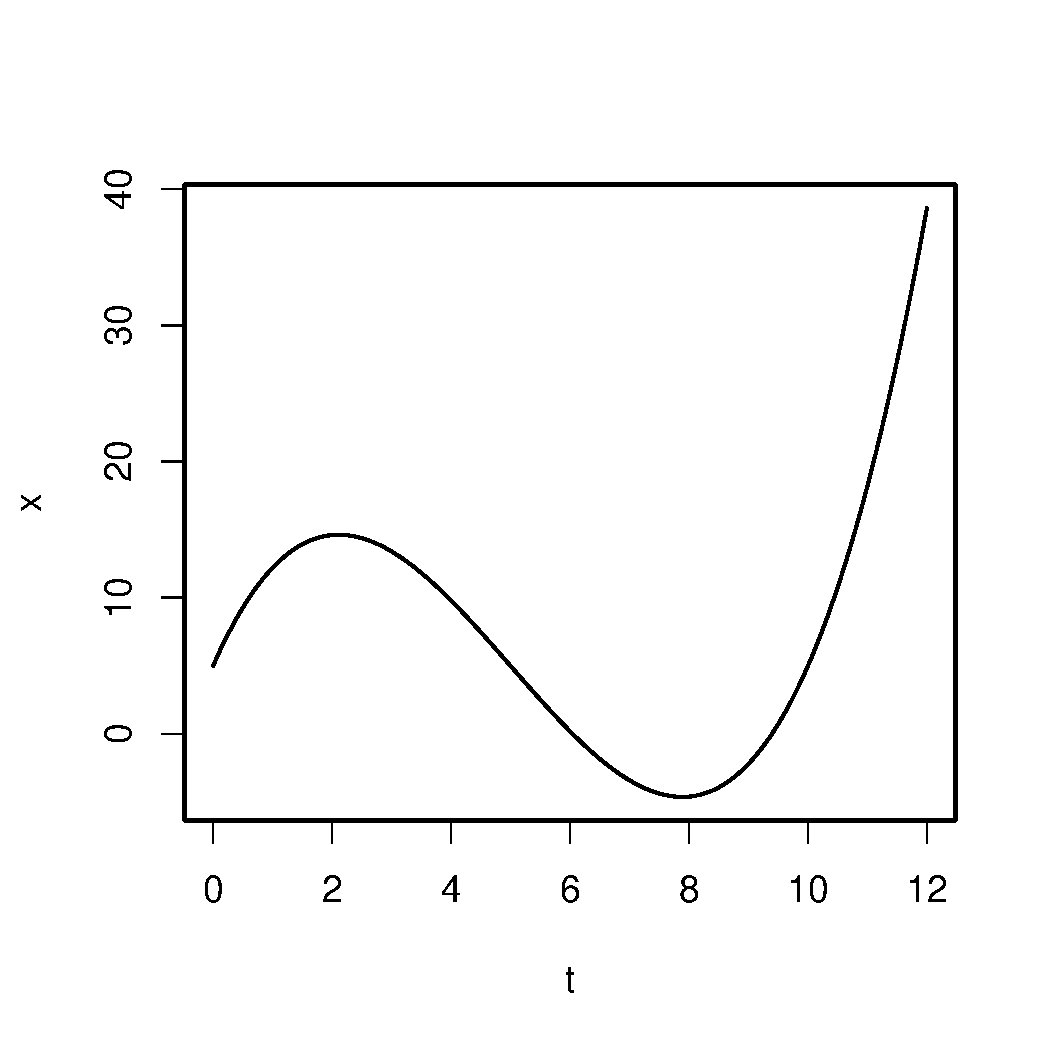
\includegraphics[width=0.7\textwidth,keepaspectratio]{fig1.pdf}
    \caption{Questão 7.}
    \label{fig:1}
  \end{figure}
\item (1,5 pontos) Suponha que o acionamento do freio de um automóvel
  provoque nele uma desaceleração constante de $20\,\un
  m/\un{s}^2$. Se o motorista do automóvel freia o carro ao observar
  que o sinal fechou, estando a uma distância de $10\,\un m$ da faixa
  de pedestres, qual deve ser a máxima velocidade do carro justo antes
  da freagem para conseguir se deter sem ultrapassar a faixa?
\item (1,5 pontos) Um automóvel se move em linha reta com uma
  velocidade constante de $30\,\un m/\un s$. Em um determinado
  instante, o motorista (distraído) do carro visualiza um caminhão na
  sua frente a uma distância de $20\,\un{m}$, o qual se move com uma
  velocidade constante de $15\,\un m/\,\un s$ na mesma direção que o
  carro. Supondo que o motorista do carro aciona o freio
  imediatamente, provocando assim uma desaceleração constante $-a_0$,
  qual deve ser o valor mínimo de $a_0$ para garantir que não haja
  colisão?

  \textit{Dica:} Se o automóvel consegue diminuir sua velocidade até
  $15\,\un m/\un s$ antes de se encontrar com o caminhão, então não
  haverá colisão. Logo, se $t_e$ é o tempo de encontro, o valor mínimo
  de $a_0$ deve ser tal que $v(t_e)=15\,\un m/\un s$.
\item (1,5 pontos) A posição de um drone em qualquer instante de tempo
  está dada pelo vetor
  $$\vec r(t)=[(3\,\un m/\un{s}^2)t^2-(4\,\un m/\un s)t]\hat i+(3\,\un m/\un s)t\hat j+[(10\,\un m/\un s)t-(2\,\un m/\un{s}^2)t^2]\hat k\,.$$
  Considerando que o eixo $z$ aponta para cima e $z=0$ corresponde ao
  nível do chão. Faça o seguinte:
  \begin{enumerate}
  \item Determine a expressão da velocidade do drone para todo
    instante de tempo.
  \item Determine a altura máxima que o drone atinge. (Nesse instante
    a componente $z$ da velocidade é nula).
  \item O drone sai do chão e retorna ao chão? Se for assim, determine
    a distância entre o ponto de saída e o ponto de retorno.
  \item Determine a expressão da aceleração do drone para todo
    instante de tempo.
  \item Determine as componentes tangencial e normal da aceleração no
    instante $t=2\,\un s$.
  \end{enumerate}
\end{enumerate}
\end{document}

